\documentclass[aspectratio=169,11pt]{beamer}

% ================================================================
% Recommendation Algorithms — Part 1 (Sami)
% Scope: hook -> explicit/implicit feedback -> rating matrix ->
%        content-based filtering -> cliffhanger into collaborative filtering
% Compile: xelatex sami_part1.tex
% 9 conceptual frames / 25 overlay pages, target ~3 minutes
% ================================================================

\usepackage{fontspec}
\setmainfont{Carlito}
\newfontfamily\headingfont{Poppins}
\newfontfamily\headingfontlight{Poppins Light}
\newfontfamily\headingfontmed{Poppins Medium}
\usepackage{microtype}
\usepackage{amsmath,amssymb,mathtools}
\usepackage{tikz}
\usetikzlibrary{arrows.meta,positioning,calc,fit,backgrounds,shapes.geometric,shapes.misc,decorations.pathreplacing,decorations.markings}
\usepackage{xcolor}
\usepackage{hyperref}

% ---------- Palette: black canvas, royal gold + emerald green ----------
\definecolor{ink}{HTML}{0D0C0A}
\definecolor{panel}{HTML}{1C1A16}
\definecolor{paneltwo}{HTML}{262219}
\definecolor{paper}{HTML}{F6F1E7}
\definecolor{muted}{HTML}{A79C89}
\definecolor{gold}{HTML}{E7B740}
\definecolor{goldeep}{HTML}{C89A2E}
\definecolor{green}{HTML}{3FA173}
\definecolor{greendeep}{HTML}{28714F}
\definecolor{rust}{HTML}{D97757}

% ---------- Beamer chrome ----------
\setbeamertemplate{navigation symbols}{}
\setbeamercolor{background canvas}{bg=ink}
\setbeamercolor{normal text}{fg=paper,bg=ink}
\setbeamercolor{frametitle}{fg=paper,bg=ink}
\setbeamercolor{framesubtitle}{fg=muted}
\setbeamerfont{title}{size=\fontsize{32}{36}}
\setbeamerfont{frametitle}{size=\fontsize{21}{25}}
\setbeamerfont{framesubtitle}{size=\fontsize{10}{12}}
\setbeamersize{text margin left=9mm,text margin right=9mm}

\setbeamertemplate{frametitle}{%
  \vspace{4mm}\hspace{-1mm}{\headingfont\bfseries\insertframetitle}\par
  \ifx\insertframesubtitle\empty\else
    \vspace{1mm}{\usebeamerfont{framesubtitle}\usebeamercolor[fg]{framesubtitle}\insertframesubtitle}\par
  \fi
}

\setbeamertemplate{footline}{%
  \begin{tikzpicture}[remember picture,overlay]
    \fill[paneltwo] (current page.south west) rectangle ([yshift=2.0mm]current page.south east);
    \pgfmathsetmacro{\progress}{\insertframenumber/max(1,\inserttotalframenumber)}
    \fill[gold] (current page.south west) rectangle ([xshift=\progress\paperwidth,yshift=2.0mm]current page.south west);
    \node[anchor=south west,font=\fontsize{5.3}{6}\selectfont,text=muted] at ([xshift=9mm,yshift=3.2mm]current page.south west) {\headingfont RECOMMENDATION ALGORITHMS \ \textbullet\ PART 1};
    \node[anchor=south east,font=\fontsize{5.3}{6}\selectfont,text=muted] at ([xshift=-9mm,yshift=3.2mm]current page.south east) {\insertframenumber/25};
  \end{tikzpicture}%
  \vspace{4.4mm}
}

% ---------- Reusable pieces ----------
\tikzset{
  flow/.style={-Latex,line width=1.3pt,draw=muted},
  flowgold/.style={-Latex,line width=1.8pt,draw=gold},
  flowgreen/.style={-Latex,line width=1.8pt,draw=green},
  card/.style={rounded corners=2.6mm,draw=white!10,fill=panel,text=paper,inner sep=4mm,align=center},
  ghostcard/.style={rounded corners=2.6mm,draw=muted!35,dashed,line width=.9pt,fill=none,text=muted,inner sep=4mm,align=center},
  dot/.style={circle,minimum size=7mm,inner sep=0pt,draw=none,fill=gold,text=ink,font=\bfseries},
  phone/.style={rounded corners=3.2mm,draw=paper,line width=1.2pt,fill=panel,minimum width=3.5cm,minimum height=6.2cm},
}
\newcommand{\hig}[1]{\textcolor{gold}{\bfseries #1}}
\newcommand{\hie}[1]{\textcolor{green}{\bfseries #1}}
\newcommand{\hir}[1]{\textcolor{rust}{\bfseries #1}}
\newcommand{\source}[1]{%
  \begin{tikzpicture}[remember picture,overlay]
    \node[anchor=south west,text=muted,font=\fontsize{4.4}{5.2}\selectfont,align=left,text width=14.5cm] at ([xshift=9mm,yshift=6.2mm]current page.south west) {#1};
  \end{tikzpicture}%
}
\newcommand{\chip}[2][gold]{%
  \tikz[baseline=(x.base)]\node[rounded corners=1.3mm,fill=#1!22!panel,draw=#1!55,text=#1,inner xsep=2.1mm,inner ysep=1.05mm,font=\fontsize{7.6}{9}\selectfont\bfseries] (x) {#2};%
}
\newcommand{\punch}[1]{{\headingfont\fontsize{19}{23}\selectfont\bfseries #1}}
\newcommand{\sectiontag}[1]{\textcolor{gold}{\headingfont\fontsize{13}{15}\selectfont\bfseries #1}}

\title{Recommendation Algorithms}
\author{Sami}
\institute{Group SS \ \textbullet\ Part 1 of 3}
\date{}

\begin{document}

% ================================================================
% F1 — Title (1 page)
% ================================================================
\begin{frame}[plain]
  \begin{tikzpicture}[remember picture,overlay]
    \fill[ink] (current page.south west) rectangle (current page.north east);
    \draw[gold!45,line width=.6pt] ([xshift=-4.6cm,yshift=-1.6cm]current page.north east) circle (2.0cm);
    \draw[green!45,line width=.9pt] ([xshift=-1.7cm,yshift=-4.7cm]current page.north east) circle (1.05cm);
    \fill[gold!70] ([xshift=-2.55cm,yshift=-1.6cm]current page.north east) circle (.045cm);
  \end{tikzpicture}
  \vspace{16mm}
  {\headingfont\fontsize{34}{38}\selectfont\bfseries\textcolor{paper}{Recommendation}\\[1mm]\textcolor{gold}{Algorithms}\par}
  \vspace{4mm}{\headingfontlight\fontsize{13}{16}\selectfont\textcolor{muted}{From one click to a ranked guess}\par}
  \vfill
  {\headingfontmed\small\textcolor{paper}{Sami}}\hspace{3mm}{\small\textcolor{muted}{\textbullet\ Part 1 of 3}}\\[1mm]
  {\scriptsize\textcolor{muted}{Group SS \ \textbullet\ Department of CSE}}
\end{frame}

% ================================================================
% F2 — Meet Bob (3 pages, cum 4)
% ================================================================
\begin{frame}{}
\centering
\vspace{4mm}
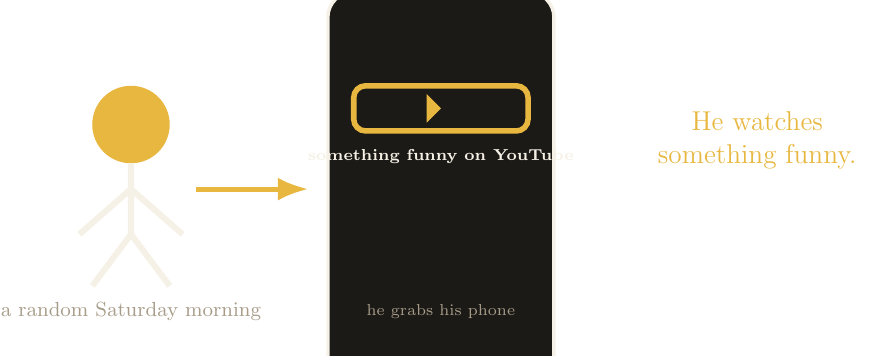
\begin{tikzpicture}[x=1cm,y=1cm,scale=.82,transform shape]
  \path[use as bounding box] (-6.4,-2.0) rectangle (6.4,2.65);
  \onslide<1->{
    \node[circle,fill=gold,minimum size=1.2cm] (head) at (-4.8,1.15) {};
    \draw[paper,line width=2.2pt,rounded corners] (-4.8,.55) -- (-4.8,-.55) (-4.8,.15) -- (-5.6,-.55) (-4.8,.15) -- (-4.0,-.55) (-4.8,-.55) -- (-5.4,-1.35) (-4.8,-.55) -- (-4.2,-1.35);
    \node[text=muted,font=\small] at (-4.8,-1.75) {a random Saturday morning};
  }
  \onslide<2->{
    \node[phone] (p) at (0,.1) {};
    \node[text=muted,font=\scriptsize] at (0,-1.75) {he grabs his phone};
    \draw[flowgold] (-3.8,.15) -- (-2.05,.15);
  }
  \onslide<3->{
    \draw[gold,line width=2pt,rounded corners=1.5mm] (-1.35,1.05) rectangle (1.35,1.75);
    \fill[gold] (0,1.4) -- (-.22,1.62) -- (-.22,1.18) -- cycle;
    \node[text=paper,font=\scriptsize\bfseries] at (0,.65) {something funny on YouTube};
    \node[gold,font=\headingfontmed\fontsize{13}{16}\selectfont] at (4.9,1.2) {He watches};
    \node[gold,font=\headingfontmed\fontsize{13}{16}\selectfont] at (4.9,.65) {something funny.};
  }
\end{tikzpicture}
\source{Illustrative scenario — no platform-specific claim.}
\end{frame}

% ================================================================
% F3 — The next morning (4 pages, cum 8)
% ================================================================
\begin{frame}{}
\centering
\vspace{3mm}
\begin{columns}[c,onlytextwidth]
  \begin{column}{.4\textwidth}
    \centering
    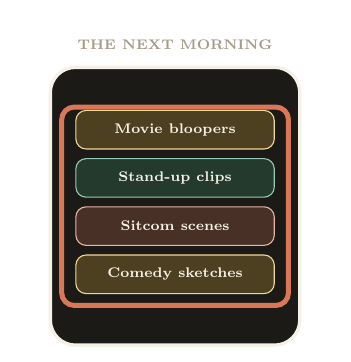
\begin{tikzpicture}[x=1cm,y=1cm,scale=.72,transform shape]
      \path[use as bounding box] (-2.6,-1.9) rectangle (2.6,3.5);
      \onslide<1->{
        \node[text=muted,font=\scriptsize\bfseries] at (0,3.2) {THE NEXT MORNING};
        \node[phone,minimum width=4.4cm,minimum height=4.9cm] (p) at (0,.35) {};
      }
      \onslide<2->{
        \foreach \y/\c/\t in {1.7/gold/{Movie bloopers},.85/green/{Stand-up clips},0/rust/{Sitcom scenes},-.85/gold/{Comedy sketches}}{
          \node[rounded corners=1.3mm,fill=\c!24!panel,draw=\c!55,minimum width=3.5cm,minimum height=.68cm,text=paper,font=\scriptsize\bfseries] at (0,\y) {\t};
        }
      }
      \onslide<3->{
        \draw[rust,line width=1.8pt,rounded corners=1.6mm] (-2.0,-1.4) rectangle (2.0,2.1);
      }
    \end{tikzpicture}
  \end{column}
  \begin{column}{.56\textwidth}
    \raggedright
    \onslide<3->{\punch{This cannot\\be a coincidence.}\\[4mm]}
    \onslide<4->{{\large\textcolor{muted}{Something happened backstage —}\\[1mm]\textcolor{muted}{we call it a }\textcolor{gold}{\bfseries recommendation system.}}}
  \end{column}
\end{columns}
\source{Illustrative scenario — no platform-specific claim.}
\end{frame}

% ================================================================
% F4 — Roadmap (2 pages, cum 10)
% ================================================================
\begin{frame}{So, let's go in depth}
\centering
\vspace{8mm}
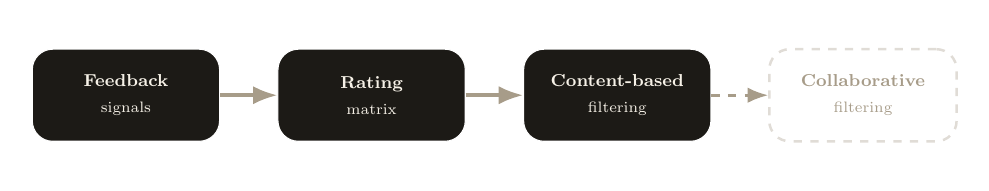
\begin{tikzpicture}[x=1cm,y=1cm,scale=.78,transform shape]
  \path[use as bounding box] (-7.6,-1.1) rectangle (7.6,1.1);
  \node[card,minimum width=3.05cm,minimum height=1.5cm] (a) at (-6.0,0) {\footnotesize\bfseries Feedback\\{\scriptsize\normalfont signals}};
  \node[card,minimum width=3.05cm,minimum height=1.5cm] (b) at (-2.0,0) {\footnotesize\bfseries Rating\\{\scriptsize\normalfont matrix}};
  \node[card,minimum width=3.05cm,minimum height=1.5cm] (c) at (2.0,0) {\footnotesize\bfseries Content-based\\{\scriptsize\normalfont filtering}};
  \node[ghostcard,minimum width=3.05cm,minimum height=1.5cm] (d) at (6.0,0) {\footnotesize\bfseries Collaborative\\{\scriptsize\normalfont filtering}};
  \draw[flow] (a)--(b); \draw[flow] (b)--(c); \draw[muted,dashed,-Latex,line width=1pt] (c)--(d);
\end{tikzpicture}
\vspace{13mm}

\onslide<2->{\textcolor{paper}{\large My three stops are here.}\ \ \textcolor{muted}{\large My friend picks up from the last one.}}
\end{frame}

% ================================================================
% F5 — Explicit vs Implicit feedback (3 pages, cum 13)
% ================================================================
\begin{frame}{How does the system learn what you like?}
\begin{columns}[T,onlytextwidth]
  \begin{column}{.48\textwidth}
    \onslide<1->{{\headingfontmed\Large\textcolor{gold}{Explicit Feedback}}\\[3mm]}
    \onslide<2->{
      
\begin{tikzpicture}
        \foreach \x in {1,...,5}{\node[star,star points=5,star point ratio=2.2,minimum size=6.5mm,fill=gold,draw=none] at (.72*\x,0) {};}
      \end{tikzpicture}\\[2mm]
      {\small\textcolor{paper}{Thumbs up/down \textbullet\ 1–5 star ratings \textbullet\ written reviews}}\\[3mm]
      {\small\textcolor{muted}{Clear signal — but rare. Most people never rate what they use.}}
    }
  \end{column}
  \begin{column}{.48\textwidth}
    \onslide<1->{{\headingfontmed\Large\textcolor{green}{Implicit Feedback}}\\[3mm]}
    \onslide<3->{
      
\begin{tikzpicture}
        \draw[paper,line width=1pt] (0,0) circle (.4cm);
        \fill[green] (-.07,-.16) -- (-.07,.16) -- (.2,0) -- cycle;
      \end{tikzpicture}\\[2mm]
      {\small\textcolor{paper}{Played songs/videos \textbullet\ purchases \textbullet\ browsing history}}\\[3mm]
      {\small\textcolor{muted}{Abundant — but noisy. A gift purchase isn't a real preference.}}
    }
  \end{column}
\end{columns}
\source{Feedback taxonomy commonly used across recommender-system literature.}
\end{frame}

% ================================================================
% F6 — The rating matrix (4 pages, cum 17)
% ================================================================
\begin{frame}{The system's core data structure}
\framesubtitle{A sparse user--item rating matrix $r_{ui}$}
\centering
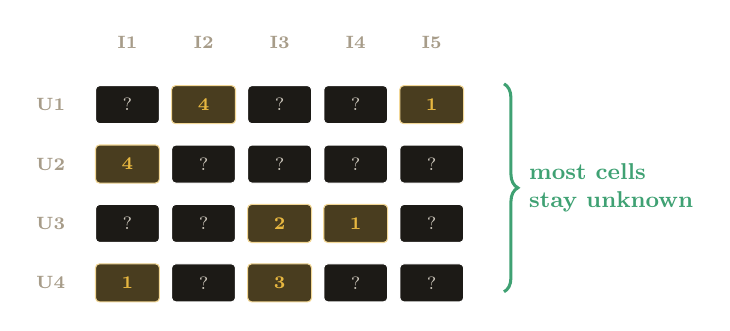
\begin{tikzpicture}[x=1.05cm,y=.82cm,scale=.92,transform shape]
  \foreach \c/\lab in {1/I1,2/I2,3/I3,4/I4,5/I5}{\node[text=muted,font=\scriptsize\bfseries] at (\c,3.05) {\lab};}
  \foreach \r/\lab in {1/U1,2/U2,3/U3,4/U4}{\node[text=muted,font=\scriptsize\bfseries,anchor=east] at (.3,3-\r) {\lab};}
  \onslide<1->{
    \foreach \c in {1,...,5}{\foreach \r in {1,...,4}{
      \draw[rounded corners=.5mm,fill=panel,draw=white!8] (\c-.42,3-\r-.32) rectangle (\c+.42,3-\r+.32);
      \node[text=muted!55,font=\scriptsize] at (\c,3-\r) {?};
    }}
  }
  \onslide<2->{
    \foreach \c/\r/\v in {2/1/4,5/1/1,1/2/4,3/3/2,4/3/1,3/4/3,1/4/1}{
      \draw[rounded corners=.5mm,fill=gold!22!panel,draw=gold!55] (\c-.42,3-\r-.32) rectangle (\c+.42,3-\r+.32);
      \node[text=gold,font=\scriptsize\bfseries] at (\c,3-\r) {\v};
    }
  }
  \onslide<3->{\draw[decorate,decoration={brace,amplitude=5pt},green,line width=1.1pt] (5.95,2.35)--(5.95,-1.15) node[midway,right=6pt,text=green,align=left,font=\small\bfseries]{most cells\\stay unknown};}
\end{tikzpicture}
\vspace{2mm}
\onslide<4->{\centering{\large\textcolor{paper}{The matrix is }\textcolor{gold}{\bfseries sparse}\textcolor{paper}{ — the algorithm must score what never happened.}}}
\source{Rating-matrix formulation standard in the recommender-systems literature (explicit $r_{ui}\in\{1,\dots,5\}$; implicit $r_{ui}\in\{0,1\}$).}
\end{frame}

% ================================================================
% F7 — Content-based filtering: concept (3 pages, cum 20)
% ================================================================
\begin{frame}{Content-based filtering describes the items}
\centering
\vspace{2mm}
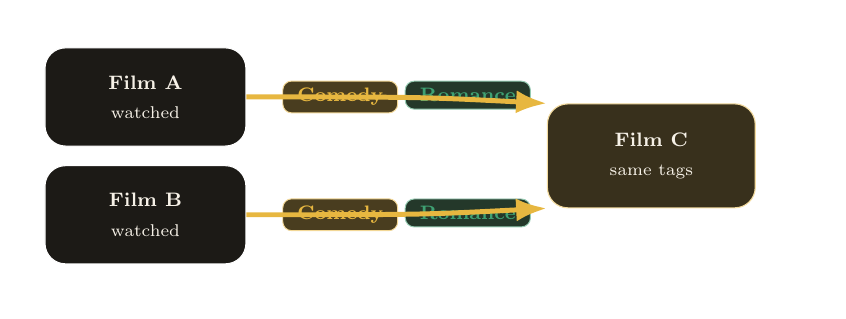
\begin{tikzpicture}[x=1cm,y=1cm,scale=.88,transform shape]
  \path[use as bounding box] (-5.7,-1.8) rectangle (5.7,2.0);
  \node<1->[card,minimum width=2.9cm,minimum height=1.4cm] (f1) at (-4.0,1.0) {\footnotesize\bfseries Film A\\{\scriptsize\normalfont watched}};
  \node<1->[card,minimum width=2.9cm,minimum height=1.4cm] (f2) at (-4.0,-.7) {\footnotesize\bfseries Film B\\{\scriptsize\normalfont watched}};
  \node<2->[anchor=west,font=\scriptsize] (t1) at (-2.15,1.0) {\chip{Comedy}\ \chip[green]{Romance}};
  \node<2->[anchor=west,font=\scriptsize] (t2) at (-2.15,-.7) {\chip{Comedy}\ \chip[green]{Romance}};
  \node<3->[card,fill=gold!14!panel,draw=gold!50,minimum width=3.0cm,minimum height=1.5cm] (f3) at (3.3,.15) {\footnotesize\bfseries Film C\\{\scriptsize\normalfont same tags}};
  \draw<3->[flowgold] (f1.east) .. controls (0,1.0) .. (f3.north west); \draw<3->[flowgold] (f2.east) .. controls (0,-.7) .. (f3.south west);
\end{tikzpicture}
\vspace{5mm}
\onslide<3->{\centering\punch{Recommend items whose profile matches yours.}}
\source{Content-based approach, matching item attributes to a user's revealed profile.}
\end{frame}

% ================================================================
% F8 — Content-based filtering: methods (3 pages, cum 23)
% ================================================================
\begin{frame}{Similarity becomes geometry}
\framesubtitle{Cosine similarity compares direction, not vector length}
\begin{columns}[c,onlytextwidth]
  \begin{column}{.54\textwidth}
    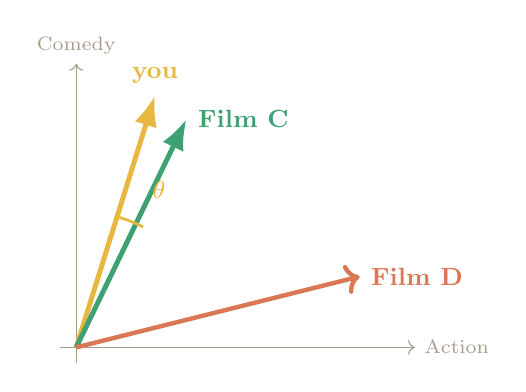
\begin{tikzpicture}[scale=1.0]
      \draw[->,muted] (-.2,0)--(4.3,0) node[right,font=\scriptsize]{Action};
      \draw[->,muted] (0,-.2)--(0,3.6) node[above,font=\scriptsize]{Comedy};
      \draw<1->[flowgold] (0,0)--(1.0,3.2) node[above,text=gold,font=\small\bfseries]{you};
      \draw<2->[flowgreen] (0,0)--(1.4,2.9) node[right,text=green,font=\small\bfseries]{Film C};
      \draw<2->[->,rust,line width=1.6pt] (0,0)--(3.6,.9) node[right,text=rust,font=\small\bfseries]{Film D};
      \draw<3->[gold,line width=1pt] (.55,1.65) arc[start angle=73,end angle=63,radius=1.85];
      \node<3->[gold,font=\small] at (1.05,2.0) {$\theta$};
    \end{tikzpicture}
  \end{column}
  \begin{column}{.42\textwidth}
    \onslide<3->{\[
      \operatorname{sim}(u,i)=\frac{u\cdot i}{\lVert u\rVert\,\lVert i\rVert}
    \]}
    \onslide<3->{\small\textcolor{muted}{small angle $\Rightarrow$ high similarity $\Rightarrow$ higher rank}\\[3mm]}
    \onslide<3->{\chip[green]{classifiers work too} \ {\scriptsize\textcolor{muted}{-- e.g. decision trees}}}
  \end{column}
\end{columns}
\source{Cosine similarity, the standard metric in content-based and neighborhood recommenders.}
\end{frame}

% ================================================================
% F9 — Cliffhanger / handoff (2 pages, cum 25)
% ================================================================
\begin{frame}{}
\centering
\vspace{4mm}
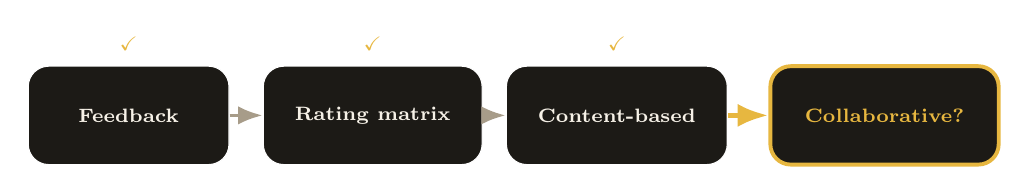
\begin{tikzpicture}[x=1cm,y=1cm]
  \onslide<1->{
  \node[card,minimum width=2.55cm,minimum height=1.25cm] (a) at (-5.0,0) {\scriptsize\bfseries Feedback};
  \node[card,minimum width=2.55cm,minimum height=1.25cm] (b) at (-1.9,0) {\scriptsize\bfseries Rating matrix};
  \node[card,minimum width=2.55cm,minimum height=1.25cm] (c) at (1.2,0) {\scriptsize\bfseries Content-based};
  \node[card,draw=gold,line width=1.4pt,minimum width=2.9cm,minimum height=1.25cm] (d) at (4.6,0) {\scriptsize\bfseries\textcolor{gold}{Collaborative?}};
  \foreach \n in {a,b,c}{\node[gold,font=\scriptsize] at ($(\n.north)+(0,.28)$) {\checkmark};}
  \draw[flow] (a)--(b); \draw[flow] (b)--(c); \draw[flowgold] (c)--(d);
  }
\end{tikzpicture}
\vspace{7mm}
\onslide<2->{\centering\punch{But what if we know nothing about the movie itself --\\no genre, no tags, nothing?}\\[3mm]
{\large\textcolor{muted}{Can we still make a good guess?}}\\[5mm]
{\headingfontmed\textcolor{gold}{Over to my friend --}}}
\end{frame}

\end{document}